\scanpage{60}
\deleted{\unsure{3}}\mspage{4}
% archive foliation: 62
Le fait que ça donne bien une structure
conforme à bord \deleted{équivalent} (qui automatiquement
redonne naissance \inserted{avec $K$} à la structure conforme
à bord $\widetilde X$ de départ) équivaut aux
\deleted{lemme suivant :}\inserted{deux cas particuliers suivants}

\deleted{\uline{Lemme 3}

a) Soit $\sigma$ un homéomorphisme rectifiable
(ou plus régulier que ça ?) de $[0,1]$ sur
lui-\deleted{\unsure{même}}, avec $\sigma(0)=0,\ \sigma(1)=1$, alors il existe
une \deleted{courbe}\inserted{\unsure{variété fermée}} $K\subset H\cap\mathbb D^\circ$,
\deleted{\unsure{bien orientée}}\inserted{avec $K\cap\delta H=\{0\}$}
\deleted{, telle que $K\setminus\{0\}$ soit contenu}
$K$ est un intervalle demi-
\deleted{dans $\operatorname{Int}H$}
ouvert d'extrémité 0 ; qui
partage $H\cap\mathbb D^\circ$ en deux comp.
\uline{connexes} $U',U''$. De plus, on trouve un

\figure{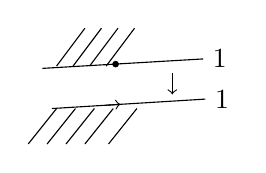
\begin{tikzpicture}[scale=.6]
\draw (-2,1.2)--(1.4,1.4);\node[right] at (1.4,1.4){$1$};
\fill(-.45,1.29)circle(2pt);
\foreach \x in {-1.7,-1.35,-1,-.65}{\draw(\x,1.25)--({\x+.6},2.05);}
\draw[->](.75,1.1)--(.75,.65);
\draw(-1.8,.35)--(1.45,.55);\node[right]at(1.45,.55){$1$};
\draw[->](-.65,.42)--(-.35,.44);
\foreach \x in {-1.7,-1.3,-.9,-.5,0}{\draw(\x,.35)--({\x-.6},-.4);}
\end{tikzpicture}}

\figure{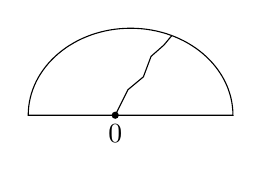
\begin{tikzpicture}[scale=.65]
\draw(-2,0)arc[start angle=180,end angle=0,x radius=2,y radius=1.7]--cycle;
\draw(-.3,0)--(-.05,.5)--(.25,.75)--(.4,1.15)--(.65,1.37)--(.8,1.55);
\fill(-.3,0)circle(2pt);\node[below]at(-.3,0){$\unsure{0}$};
\end{tikzpicture}}
}

\uline{Lemme 3} Cas particuliers

a) Recollement de $H$ à $H$ \inserted{(\uline{deux exemplaires})} suivant un
iso. rectifiable $[0,1]\unsure{\mathrel{\overset{\sigma}{-}}|\xrightarrow{\sigma}}[0,1]$, regardé au
voisinage de 0 [ou variante (\unsure{pour}\ \deleted{\unsure{des}} établir
th. 3) : suivant un isom rectifiable $[-1,1]\xrightarrow{\sigma}[-1,1]$,
regardé au voisinage de 0].
